% Options for packages loaded elsewhere
\PassOptionsToPackage{unicode}{hyperref}
\PassOptionsToPackage{hyphens}{url}
\documentclass[
  a4paper,11pt]{article}
\usepackage{xcolor}
\usepackage[margin=1in]{geometry}
\usepackage{amsmath,amssymb}
\usepackage{graphicx}
\setcounter{secnumdepth}{-\maxdimen} % remove section numbering
\usepackage{iftex}
\ifPDFTeX
  \usepackage[T1]{fontenc}
  \usepackage[utf8]{inputenc}
  \usepackage{textcomp} % provide euro and other symbols
\else % if luatex or xetex
  \usepackage{unicode-math} % this also loads fontspec
  \defaultfontfeatures{Scale=MatchLowercase}
  \defaultfontfeatures[\rmfamily]{Ligatures=TeX,Scale=1}
\fi
\usepackage{lmodern}
\ifPDFTeX\else
  % xetex/luatex font selection
  \setmainfont[]{Times New Roman}
\fi
% Use upquote if available, for straight quotes in verbatim environments
\IfFileExists{upquote.sty}{\usepackage{upquote}}{}
\IfFileExists{microtype.sty}{% use microtype if available
  \usepackage[]{microtype}
  \UseMicrotypeSet[protrusion]{basicmath} % disable protrusion for tt fonts
}{}
\makeatletter
\@ifundefined{KOMAClassName}{% if non-KOMA class
  \IfFileExists{parskip.sty}{%
    \usepackage{parskip}
  }{% else
    \setlength{\parindent}{0pt}
    \setlength{\parskip}{6pt plus 2pt minus 1pt}}
}{% if KOMA class
  \KOMAoptions{parskip=half}}
\makeatother
\usepackage{longtable,booktabs,array}
\newcounter{none} % for unnumbered tables
\usepackage{calc} % for calculating minipage widths
% Correct order of tables after \paragraph or \subparagraph
\usepackage{etoolbox}
\makeatletter
\patchcmd\longtable{\par}{\if@noskipsec\mbox{}\fi\par}{}{}
\makeatother
% Allow footnotes in longtable head/foot
\IfFileExists{footnotehyper.sty}{\usepackage{footnotehyper}}{\usepackage{footnote}}
\makesavenoteenv{longtable}
\setlength{\emergencystretch}{3em} % prevent overfull lines
\providecommand{\tightlist}{%
  \setlength{\itemsep}{0pt}\setlength{\parskip}{0pt}}
\usepackage{bookmark}
\IfFileExists{xurl.sty}{\usepackage{xurl}}{} % add URL line breaks if available
\urlstyle{same}
\hypersetup{
  hidelinks,
  pdfcreator={LaTeX via pandoc}}

\author{}
\date{}

\begin{document}

\section{\texorpdfstring{Three-Layer Projection Model: Nested Subjective
Spaces \(R\)--\(R_1\)--\(R_0\) and Middleware Geometry via Central
Projection}{Three-Layer Projection Model: Nested Subjective Spaces R--R\_1--R\_0 and Middleware Geometry via Central Projection}}\label{three-layer-projection-model-nested-subjective-spaces-rr_1r_0-and-middleware-geometry-via-central-projection}

\textbf{Author}: Noriaki Kihara\\
\textbf{Affiliation}: WF System Co., Ltd.\\
\textbf{ORCID}: 0009-0004-6753-4020\\
\textbf{Version}: v1.0\\
\textbf{DOI}:
\href{https://doi.org/10.5281/zenodo.19691713}{10.5281/zenodo.19691713}\\
\textbf{Date}: April 2026

\begin{center}\rule{0.5\linewidth}{0.5pt}\end{center}

\subsection{Abstract}\label{abstract}

This paper organizes and integrates the geometric properties of
subjective spaces, already established in the central projection series,
into a \textbf{three-layer structure \(R\)--\(R_1\)--\(R_0\)} as a
middleware paper. It proves no new theorems and confines itself to
observing the following structure as a combination of known properties
of central projection:

\begin{enumerate}
\def\labelenumi{\arabic{enumi}.}
\tightlist
\item
  For any curvature radius \(R\), the subjective space \(S^n(R)\) is
  defined as a central projection centered at the common origin \(O\) of
  the background coordinate space.
\item
  Two subjective spaces \(S^n(R_1)\) and \(S^n(R_0)\) at different
  scales are arranged as a concentric nested structure by virtue of
  origin sharing and projection-axis collinearity.
\item
  The \(R\)-direction displacement connecting corresponding points on
  different subjective spaces is orthogonal to the tangent spaces of all
  subjective spaces and hence cannot be measured by any intrinsic
  metric.
\end{enumerate}

This structure provides an \textbf{implementation-independent stable
interface} for \textbf{upper and lower implementation layers} in which
each particle may possess its own subjective space as a micro black
hole. This paper relies on neither the specific implementation of
particle internal structure nor the specific implementation of
phase-space dynamics, and its scope of claims is limited to the
geometric middleware connecting the two.

\textbf{Keywords}: central projection, subjective space, background
coordinate preservation, origin sharing, concentric structure, metric
non-contribution of \(R\)-direction displacement, middleware geometry

\begin{center}\rule{0.5\linewidth}{0.5pt}\end{center}

\subsection{§1 Scope of Claims and Separation
Principle}\label{scope-of-claims-and-separation-principle}

The claims of this paper are limited to the \textbf{organization and
integration} of properties established in the central projection series
foundational papers {[}P1{]}, {[}P2{]}, {[}P8{]}. No new mathematical
claims are made.

The following elements are \textbf{outside the scope of this paper's
claims} and are treated only as implementation examples when mentioned
in the text:

\begin{itemize}
\tightlist
\item
  Specific implementations of particle internal structure (including the
  6-dimensional hyperrectangle model {[}W8{]})
\item
  Phase-space dynamics inside micro black holes (including soliton wave
  equations)
\item
  Correspondence with individual particles in the Standard Model
\end{itemize}

The claims of this paper are unaffected even if the above
implementations are entirely incorrect, as long as the paper relies on
the geometric properties of central projection themselves. This follows,
at a higher layer, the policy of ``separation of mathematical substance
and interpretation'' in {[}W8{]}.

\begin{center}\rule{0.5\linewidth}{0.5pt}\end{center}

\subsection{§2 Basic Conditions and
Constraints}\label{basic-conditions-and-constraints}

The three-layer structure of this paper is defined under the following
conditions.

\subsubsection{Condition 1 (Origin
Sharing)}\label{condition-1-origin-sharing}

All subjective spaces \(S^n(R)\), \(S^n(R_1)\), \(S^n(R_0)\) share the
\textbf{same origin \(O\)} of the background coordinate space
\(\mathbb{R}^{n+1}\) as the projection center of central projection.
This is a structural condition that follows directly from the definition
of central projection (§3.1) and is not an additional assumption.

\subsubsection{Condition 2 (Sharing of Axis
Directions)}\label{condition-2-sharing-of-axis-directions}

For any subjective space with \(R > 0\), the \textbf{directions of the
half-lines} (projection axes) emanating from the origin \(O\) of the
background coordinate space \textbf{are shared}. That is, even when the
curvature radius \(R\) differs, the directional structure of the
projection axes is identical. This also follows directly from the
definition of central projection in §3.1 (\(R > 0\)).

\subsubsection{Condition 3 (Non-constraint on
Multiplicity)}\label{condition-3-non-constraint-on-multiplicity}

There is \textbf{no upper bound on the number} of general subjective
spaces \(S^n(R)\) and particle-scale subjective spaces \(S^n(R_1)\).
Subjective spaces sharing the same origin \(O\) may exist infinitely,
one for each distinct curvature radius. This follows from the fact that
the definition of central projection holds for any value of curvature
radius \(R > 0\).

\subsubsection{\texorpdfstring{Condition 4 (On the Uniqueness of
\(R_0\))}{Condition 4 (On the Uniqueness of R\_0)}}\label{condition-4-on-the-uniqueness-of-r_0}

In this paper, since \(S^n(R_0)\) is treated as the subjective space
corresponding to the 4-dimensional spacetime we observe, \(R_0\) is
\textbf{assumed to be unique}. However, this is \textbf{not a
constraint} on the geometric claims of this paper. Even if multiple (or
infinitely many) subjective spaces corresponding to \(R_0\) existed, the
claims of §3--§6 would not break down. The uniqueness of \(R_0\) is a
conventional setting reflecting our observational standpoint.

The above conditions are illustrated below.

\begin{figure}[htbp]
\centering
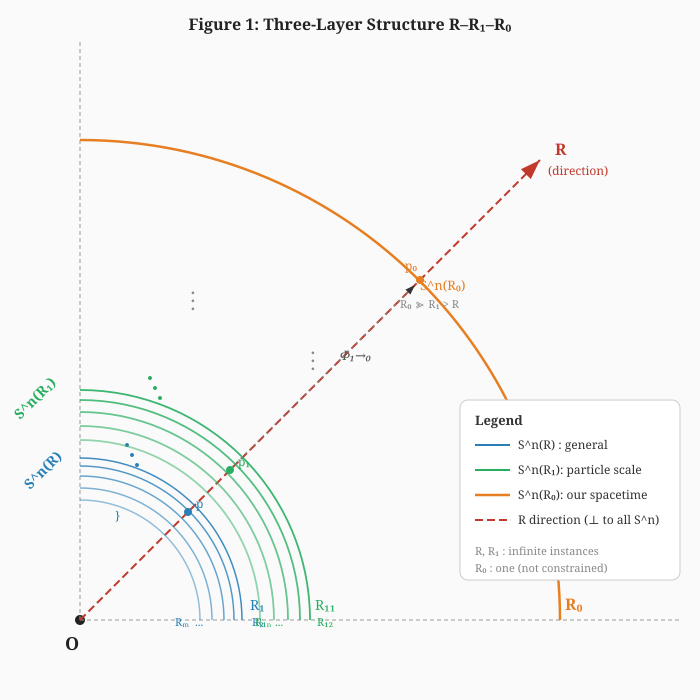
\includegraphics[width=0.7\textwidth]{fig1_three_layer_structure.pdf}
\caption{Conceptual diagram of the three-layer structure, drawn as quarter circles sharing the origin $O$. The blue arc group $S^n(R)$ and the green arc group $S^n(R_1)$ may each have infinitely many instances (Condition 3). The orange arc $S^n(R_0)$ is our subjective space (Condition 4). The red dashed line indicates the $R$-direction, which is orthogonal to the tangent spaces of all $S^n$. The points $p$, $p_1$, $p_0$ shown on the 45-degree half-line are corresponding points on the same background coordinate half-line, connected by the map $\Phi_{1 \to 0}$ (the 45-degree direction is a drawing convenience; the same correspondence holds for half-lines in any direction).}
\end{figure}

\begin{center}\rule{0.5\linewidth}{0.5pt}\end{center}

\subsection{§3 Prerequisites: Basic Properties of Central Projection
(Cited)}\label{prerequisites-basic-properties-of-central-projection-cited}

This section contains no new claims. It organizes the basic properties
used in subsequent discussion by citing them from the foundational
papers.

\subsubsection{§3.1 Definition of Central
Projection}\label{definition-of-central-projection}

With the origin \(O\) of the background coordinate space
\(\mathbb{R}^{n+1}\) as the projection center, the central projection
onto the hypersphere \(S^n(R) \subset \mathbb{R}^{n+1}\) with curvature
radius \(R > 0\) is defined as

\[
P_R : \mathbb{R}^{n+1} \setminus \{O\} \to S^n(R), \quad P_R(\mathbf{x}) = R \cdot \frac{\mathbf{x}}{\|\mathbf{x}\|}
\]

({[}P1{]} §2). The image \(S^n(R)\) of \(P_R\) is called the
\textbf{subjective space of curvature radius \(R\)}.

\subsubsection{§3.2 Background Coordinate
Preservation}\label{background-coordinate-preservation}

The central projection \(P_R\) \textbf{preserves background coordinates}
({[}P1{]} §3). That is, the original half-line in background coordinates
can be uniquely recovered from the projection image via the inverse
projection, and this correspondence is regular.

\subsubsection{§3.3 Observability within the Subjective
Space}\label{observability-within-the-subjective-space}

The quantities measurable by an observer inside the subjective space
\(S^n(R)\) are limited to geodesic lengths and winding numbers on
\(S^n(R)\). In particular, the distance in the radial direction
(\(R\)-direction) \textbf{cannot be perceived} from inside the
subjective space ({[}P2{]} §4, {[}P8{]} §3).

\begin{center}\rule{0.5\linewidth}{0.5pt}\end{center}

\subsection{§4 Definition of the Three-Layer
Structure}\label{definition-of-the-three-layer-structure}

\subsubsection{§4.1 Roles of the Three
Symbols}\label{roles-of-the-three-symbols}

In this paper, the following three symbols are used as curvature radii
defined by central projection.

\begin{itemize}
\tightlist
\item
  \(R\): A \textbf{generic symbol} denoting the curvature radius of the
  subjective space \(S^n(R)\). The definition parameter of central
  projection as defined in §3.
\item
  \(R_1\): A \textbf{specific instance} denoting the curvature radius of
  the particle-scale subjective space \(S^n(R_1)\). In the upper
  implementation layer (see §7), it may be interpreted as the curvature
  radius of a micro black hole.
\item
  \(R_0\): A \textbf{specific instance} denoting the curvature radius of
  our subjective space \(S^n(R_0)\). A nearly flat subjective space with
  \(R_0 \to \infty\).
\end{itemize}

\textbf{Note}: Within the scope of this paper, \(R\) is a generic
symbol, and \(R_1\) and \(R_0\) are two instances that specialize it.
The implementation that identifies \(R = R_1\) is presented in §7
(Implementation Examples), but the claims of this paper do not depend on
this identification.

\subsubsection{§4.2 Claims on the Three-Layer
Structure}\label{claims-on-the-three-layer-structure}

\textbf{Claim 4.1 (Origin Sharing)}: For any curvature radius \(R\), the
subjective space \(S^n(R)\) is defined by central projection centered at
the \textbf{same origin \(O\)} of the background coordinates, by the
definition in §3.1. Therefore, \(S^n(R_1)\) and \(S^n(R_0)\) share the
common origin \(O\).

\textbf{Basis}: Directly from the definition of central projection in
{[}P1{]} §2. No new proof is needed.

\textbf{Claim 4.2 (Projection-Axis Collinearity)}: Any half-line
emanating from the origin \(O\) of the background coordinate space
passes through both \(S^n(R_1)\) and \(S^n(R_0)\) in the \textbf{same
direction}.

\textbf{Basis}: Directly from the background coordinate preservation
property in {[}P1{]} §3. No new proof is needed.

\textbf{Claim 4.3 (Concentric Nested Structure)}: From Claims 4.1 and
4.2, \(S^n(R_1)\) and \(S^n(R_0)\) are arranged as \textbf{concentric
nested shells} sharing the same axial structure, centered at the origin
\(O\).

\textbf{Basis}: A trivial consequence of the combination of Claims 4.1
and 4.2.

\begin{center}\rule{0.5\linewidth}{0.5pt}\end{center}

\subsection{\texorpdfstring{§5 Orthogonality of the \(R\)-Direction and
Metric
Non-Contribution}{§5 Orthogonality of the R-Direction and Metric Non-Contribution}}\label{orthogonality-of-the-r-direction-and-metric-non-contribution}

\subsubsection{\texorpdfstring{§5.1 Orthogonality of the
\(R\)-Direction}{§5.1 Orthogonality of the R-Direction}}\label{orthogonality-of-the-r-direction}

Since \(S^n(R)\) is a hypersphere of radius \(R\) centered at the origin
\(O\) in the background coordinate space \(\mathbb{R}^{n+1}\), at any
point \(p \in S^n(R)\) the radial direction (\(R\)-direction) is
\textbf{orthogonal} to the tangent space \(T_p S^n(R)\) of \(S^n(R)\).
Therefore, displacement in the \(R\)-direction \textbf{does not
contribute} to the induced metric on \(S^n(R)\).

\subsubsection{§5.2 Metric
Non-Contribution}\label{metric-non-contribution}

\textbf{Claim 5.1 (Metric Non-Contribution of \(R\)-Direction
Displacement)}: On any half-line \(\ell\) emanating from the origin
\(O\) of the background coordinate space, a point \(p_1\) on
\(S^n(R_1)\) and a point \(p_0\) on \(S^n(R_0)\) correspond to each
other. The \(R\)-direction displacement connecting \(p_1\) and \(p_0\)
is orthogonal to the tangent space of \(S^n(R_0)\) and hence
\textbf{does not contribute} to the geodesic metric on \(S^n(R_0)\).
Similarly, it does not contribute to the geodesic metric on
\(S^n(R_1)\). Therefore, the \(R\)-direction distance between \(p_1\)
and \(p_0\) \textbf{cannot be measured by the intrinsic metric of any
subjective space}.

\textbf{Basis}: An observation from the combination of the orthogonality
in §5.1 and Claim 4.2. No new proof is needed.

\textbf{Remark 1}: This claim does not mean that \(p_1\) and \(p_0\) are
the same point from the external viewpoint of the background coordinate
space, or that the distance between them is zero. From the external
viewpoint, they are at different radial positions. The claim is confined
to the geometric fact that the \(R\)-direction displacement connecting
\(p_1\) and \(p_0\) is orthogonal to the tangent spaces of the
subjective spaces, and hence \textbf{the distance in that direction does
not contribute to the metric}.

\textbf{Remark 2}: This claim does \textbf{not} mean that the values of
the curvature radii \(R_0\), \(R_1\) themselves cannot be perceived from
inside the subjective space. Since the curvature radius \(R\) determines
the geodesic curvature of \(S^n(R)\), a change in the value of \(R\)
alters the internal geodesic structure (curvature distortion), which is
perceptible to an internal observer. What this claim states is the more
limited fact that the \textbf{\(R\)-direction distance} between
corresponding points on different subjective spaces cannot be measured.

\subsubsection{§5.3 Inter-Layer Map via Central
Projection}\label{inter-layer-map-via-central-projection}

For any point \(p_1\) on \(S^n(R_1)\), the map that assigns the
intersection \(p_0\) of the half-line from the origin \(O\) through
\(p_1\) with \(S^n(R_0)\),

\[
\Phi_{1 \to 0} : S^n(R_1) \to S^n(R_0), \quad \Phi_{1 \to 0}(p_1) = P_{R_0}(P_{R_1}^{-1}(p_1))
\]

is well-defined and regular.

\textbf{Basis}: Directly from the central projection definition in §3.1
and the background coordinate preservation in §3.2.

\textbf{Note}: \(P_{R_1}\) is a surjection from
\(\mathbb{R}^{n+1} \setminus \{O\}\) to \(S^n(R_1)\) and is not
injective (all points on the same half-line project to a single point).
Here \(P_{R_1}^{-1}(p_1)\) refers to the entire half-line that projects
to \(p_1\). By the background coordinate preservation of §3.2, this
half-line is uniquely recovered from \(p_1\), and applying \(P_{R_0}\)
yields the unique image \(p_0\) on \(S^n(R_0)\), so \(\Phi_{1 \to 0}\)
is well-defined.

\begin{center}\rule{0.5\linewidth}{0.5pt}\end{center}

\subsection{§6 Summary of Claims}\label{summary-of-claims}

The geometric structure claimed by this paper is exhausted by the
following.

\begin{enumerate}
\def\labelenumi{\arabic{enumi}.}
\tightlist
\item
  Any subjective space defined by central projection shares the origin
  of the background coordinates (§4.2, Claim 4.1).
\item
  Subjective spaces of different curvature radii are arranged as a
  concentric nested structure (§4.2, Claim 4.3).
\item
  The \(R\)-direction displacement connecting corresponding points on
  different subjective spaces is orthogonal to the tangent spaces of all
  subjective spaces, and hence the distance in that direction cannot be
  measured by any intrinsic metric (§5.2, Claim 5.1).
\item
  The inter-layer map via central projection between subjective spaces
  is well-defined and regular (§5.3).
\end{enumerate}

All of these are properties derived directly from the foundational
papers {[}P1{]}, {[}P2{]}, {[}P8{]}, and this paper bears no independent
proof burden.

The originality of this paper lies in the \textbf{viewpoint of
integrating these known properties as a middleware structure}. Namely,
by hierarchizing \(R\) as a generic symbol and \(R_1\) and \(R_0\) as
its instances, and positioning central projection as the interface
connecting them, we obtain a \textbf{stable geometric framework
independent of specific implementations of internal structure}.

\begin{center}\rule{0.5\linewidth}{0.5pt}\end{center}

\subsection{§7 Implementation Examples (Not Claims of This
Paper)}\label{implementation-examples-not-claims-of-this-paper}

\textbf{The content of this section is not a claim of this paper but an
example of concretizing the three-layer structure model.} Even if the
implementations mentioned in this section (6-dimensional hyperrectangle,
soliton waves, micro black hole interpretation, etc.) are incorrect, the
claims of §3--§6 are unaffected.

\subsubsection{§7.1 Lower-Layer Implementation Example: Particle
Internal
Structure}\label{lower-layer-implementation-example-particle-internal-structure}

An implementation can be considered in which \(R = R_1\) is identified
and each particle is treated as a closed geometric object possessing its
own subjective space \(S^n(R_1)\). In this implementation, the internal
structure of a particle is described as a combinatorial structure inside
\(S^n(R_1)\). A concrete example is the 6-dimensional hyperrectangle
model of {[}W8{]} (classification of 62 particles by axis orientation of
xyztRQ).

This paper does not claim that this implementation is correct. The
geometric structure of central projection holds equally whether the
interior of a particle is a 6-dimensional hyperrectangle or any other
combinatorial structure.

\subsubsection{§7.2 Upper-Layer Implementation Example: Location of
Phase
Space}\label{upper-layer-implementation-example-location-of-phase-space}

An implementation can be considered in which the phase space of a
particle as a soliton wave is located inside \(S^n(R_1)\). In this
implementation, the position and phase information of each particle
instance in a many-body problem is held inside its respective
\(S^n(R_1)\). On the \(S^n(R_0)\) side, only observational information
appears as an image via central projection.

This paper does not claim that this implementation is correct. As an
alternative regarding the location of phase space, structurally one
could also consider an arrangement in which the \(S^n(R_0)\) side holds
the phase space. The author considers the former arrangement, combined
with the implementation of §7.1, to be more natural, but this preference
is not a claim of this paper.

\subsubsection{§7.3 Micro Black Hole
Interpretation}\label{micro-black-hole-interpretation}

An interpretation can be considered in which \(S^n(R_1)\) is interpreted
as a particle-scale micro black hole subjective space, and particle
properties are described as an extension of the general-relativistic
no-hair theorem. In this interpretation, to an internal observer of
\(S^n(R_0)\), the micro black hole appears as a central projection image
(a point-like projection), and the internal structure is confined behind
the event horizon.

This paper does not claim that this interpretation is correct. The
interpretation is merely one reading of the geometric structure of
central projection, and other interpretations are not excluded.

\subsubsection{§7.4 Implementation Example of Interaction
Mechanism}\label{implementation-example-of-interaction-mechanism}

An implementation can be considered that interprets the metric
non-contribution of the \(R\)-direction displacement in §5.2 as a
geometric mechanism for interaction between different particles
(different \(S^n(R_1)\) instances). When two particle subjective spaces
\(S^n(R_1^{(A)})\) and \(S^n(R_1^{(B)})\) have an \(R\)-direction
connection that is unmeasurable by intrinsic metric on the same
background coordinate half-line, an interaction channel opens between
them.

This paper does not address the dynamical details of this
implementation. The specific equations of interaction, coupling
constants, and the role of mediating particles are deferred to future
papers.

\begin{center}\rule{0.5\linewidth}{0.5pt}\end{center}

\subsection{§8 Conclusion}\label{conclusion}

This paper is a middleware paper that organizes and integrates the
geometric properties of subjective spaces established in the central
projection series foundational papers {[}P1{]}, {[}P2{]}, {[}P8{]} as a
three-layer structure \(R\)--\(R_1\)--\(R_0\). Without proving new
theorems, the following structure was observed as a combination of known
properties:

\begin{itemize}
\tightlist
\item
  All subjective spaces share the common origin of the background
  coordinates
\item
  Subjective spaces of different curvature radii are arranged as
  concentric nested shells
\item
  The \(R\)-direction displacement connecting corresponding points on
  different subjective spaces is orthogonal to the tangent spaces of all
  subjective spaces, and hence the distance in that direction cannot be
  measured by intrinsic metric
\item
  The inter-layer map via central projection between subjective spaces
  is well-defined and regular
\end{itemize}

This structure is independent of specific implementations such as
particle internal structure and phase-space dynamics, and is positioned
as a \textbf{middleware geometry} that remains stable even when the
implementations of the upper and lower layers are changed.

In future papers, specific implementations of particle internals
(6-dimensional hyperrectangle model, etc.) and phase-space dynamics
(soliton wave model, etc.) will be built step by step on top of this
middleware structure. Each implementation paper will be developed as an
independent object of verification while presupposing the geometric
foundation of this paper.

\textbf{Position within the series}: This paper is positioned between
the central projection series foundational paper group (Papers 1--10)
and the phase equation series (W1--W9). It integrates the individual
geometric properties established by the foundational paper group into a
three-layer structure and provides a stable interface on which the
implementations of the phase equation series can rest.

\subsubsection{§8.1 Explicit Statement of What This Paper Does Not
Claim}\label{explicit-statement-of-what-this-paper-does-not-claim}

To prevent misreading, the following are explicitly stated.

\begin{itemize}
\tightlist
\item
  \textbf{Does not claim the existence of micro black holes.} Although
  §7.3 mentions the micro black hole interpretation, this is one reading
  (implementation example) of the three-layer structure, and this paper
  does not contain the claim that micro black holes physically exist.
\item
  \textbf{Does not claim many-worlds interpretation or many-worlds
  hypothesis.} The ``nested structure'' of this paper describes the
  geometric property of central projection that concentric spheres are
  arranged, and is unrelated to the many-worlds interpretation (Everett
  interpretation) in quantum mechanics or similar claims.
\item
  \textbf{Does not claim that particles are condensed in the limit
  \(R \to 0\).} This paper states that \(R_1\) is smaller than \(R_0\),
  but does not perform the limiting operation \(R \to 0\). The picture
  of particles being condensed to a point is not included in the claims
  of this paper.
\end{itemize}

\begin{center}\rule{0.5\linewidth}{0.5pt}\end{center}

\subsection{References}\label{references}

\subsubsection{Cited in the main body
(§3--§6)}\label{cited-in-the-main-body-36}

\begin{itemize}
\tightlist
\item
  {[}P1{]}: Noriaki Kihara, Geometric Formulation of 4-Dimensional Space
  via Central Projection, Zenodo, 2026. DOI:
  \href{https://doi.org/10.5281/zenodo.19427780}{10.5281/zenodo.19427780}
\item
  {[}P2{]}: Noriaki Kihara, Geometric Symmetry of Central Projection:
  Mathematical Foundation of Multi-Axis Models, Zenodo, 2026. DOI:
  \href{https://doi.org/10.5281/zenodo.19434932}{10.5281/zenodo.19434932}
\item
  {[}P8{]}: Noriaki Kihara, Diameter of the Circumscribed Hypersphere of
  a Unit-Volume 4-Dimensional Hyperrectangle, Zenodo, 2026. DOI:
  \href{https://doi.org/10.5281/zenodo.19533313}{10.5281/zenodo.19533313}
\end{itemize}

\subsubsection{Cited in implementation examples
(§7)}\label{cited-in-implementation-examples-7}

\begin{itemize}
\tightlist
\item
  {[}W8{]}: Noriaki Kihara, Set-Theoretic Structure and Combinatorial
  Properties of 6-Dimensional Hyperrectangles (v5), Zenodo, 2026. DOI:
  \href{https://doi.org/10.5281/zenodo.19688521}{10.5281/zenodo.19688521}
\end{itemize}

\subsubsection{Other}\label{other}

\begin{itemize}
\tightlist
\item
  Source code: https://github.com/WurabeSeiji/ai-chat-logs-open/
\end{itemize}

\begin{center}\rule{0.5\linewidth}{0.5pt}\end{center}

\subsection{Appendix A: Self-Check on the Scope of This
Paper}\label{appendix-a-self-check-on-the-scope-of-this-paper}

As a self-check of the writing policy, it is explicitly stated that the
claims of this paper are unaffected in any of the following cases.

{\def\LTcaptype{none} % do not increment counter
\begin{longtable}[]{@{}
  >{\raggedright\arraybackslash}p{(\linewidth - 2\tabcolsep) * \real{0.8621}}
  >{\raggedright\arraybackslash}p{(\linewidth - 2\tabcolsep) * \real{0.1379}}@{}}
\toprule\noalign{}
\begin{minipage}[b]{\linewidth}\raggedright
Hypothetical scenario that does not affect claims
\end{minipage} & \begin{minipage}[b]{\linewidth}\raggedright
Reason
\end{minipage} \\
\midrule\noalign{}
\endhead
\bottomrule\noalign{}
\endlastfoot
The 6-dimensional hyperrectangle model {[}W8{]} is found to be entirely
incorrect & §7.1 is an implementation example, independent of the claims
in §3--§6 \\
The soliton wave model is found to be entirely incorrect & §7.2 is an
implementation example, independent of the claims in §3--§6 \\
The micro black hole interpretation is found to be physically
inappropriate & §7.3 is an interpretation example, independent of the
claims in §3--§6 \\
Correspondence with individual particles in the Standard Model is found
to be invalid & This paper does not claim individual particle
correspondence \\
\end{longtable}
}

The claims of this paper hold in any of the above scenarios, as long as
the foundational papers {[}P1{]}, {[}P2{]}, {[}P8{]} remain
mathematically valid.

\begin{center}\rule{0.5\linewidth}{0.5pt}\end{center}

\emph{v1.0}

\end{document}
